\subsection{Itinerary Optimisation Algorithms}

We tested out the itinerary generation algorithm using
POIs in Malta. The algorithm has to optimise to
produce the best itinerary for X number and several
tourist constraints. Figure \ref{optimise} shows the score of 10
PSO itineraries increasing throughout several
iterations for the morning and evening section of the
day.

\begin{figure}[h]
\centering
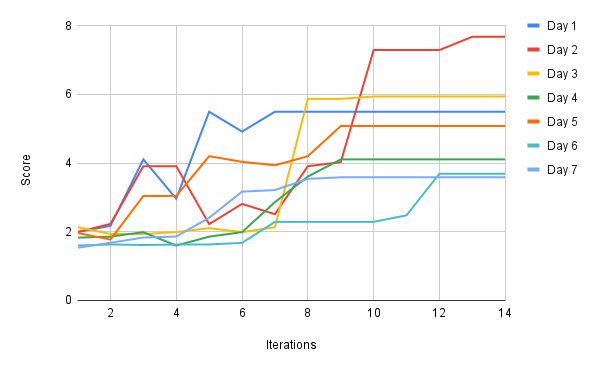
\includegraphics[width=0.7\textwidth]{Optimisation.png}
\caption{Training and validation accuracy of the model on the testing and validation dataset}
\label{optimise}
\end{figure}

Many parameters help tweak the performance of the PSO
algorithm. The population size and the number of
iterations are the two main attributes of the PSO
algorithm. At around 12 iterations in figure~\ref{optimise}, the
algorithm generally converges. Figure X shows the
spread of particles converging. 


Increasing the number of particles also increases the
average score, as shown in figure~\ref{score} for 10 generated
itineraries and 14 iterations. However, the difference
in average score between 50 and 100 particles is not
proportional to the average time taken to create an
itinerary for a single day in figure~\ref{time}.  That is why
for the application, the population is set to 50. 

\begin{figure}[h]
\centering
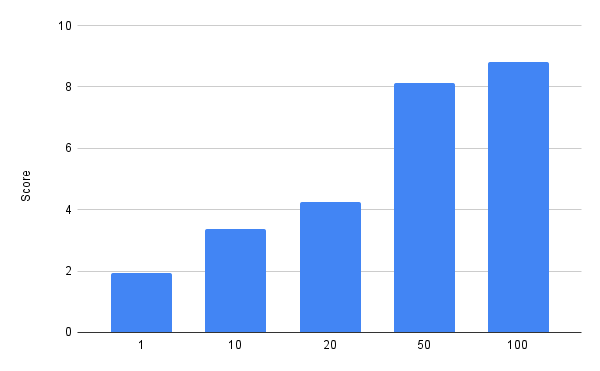
\includegraphics[width=0.7\textwidth]{Score.png}
\caption{Training and validation accuracy of the model on the testing and validation dataset}
\label{score}
\end{figure}

\begin{figure}[h]
\centering
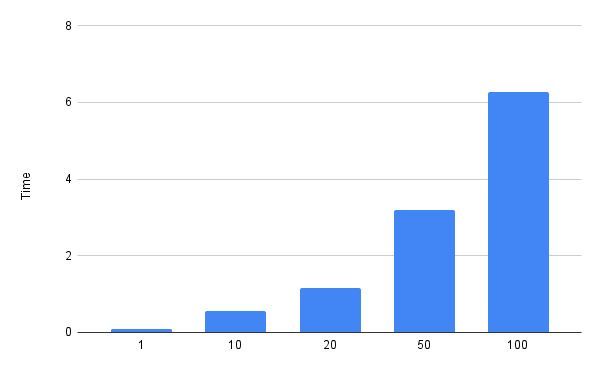
\includegraphics[width=0.7\textwidth]{Time.png}
\caption{Training and validation accuracy of the model on the testing and validation dataset}
\label{time}
\end{figure}

The original algorithm X did not contain the inertia
property; however, it was introduced by X since it
controls the convergence behaviour. Out algorithm
implements the Time-Varying Inertia Weight X, which
gradually decreases throughout each iteration. Figure
X shows the optimisation algorithm without the inertia
property and barely increases the score since the
particles do not explore new territories.
